\documentclass[11pt,a4paper]{article}

% =========================================================================
% PAKET-PAKET UTAMA & PENGATURAN TATA LETAK
% =========================================================================
\usepackage[utf8]{inputenc}
\usepackage[T1]{fontenc}
\usepackage{lmodern}
\usepackage[indonesian]{babel}
\usepackage{amsmath,amssymb,amsfonts,amsthm}
\usepackage{bm}
\usepackage{geometry}
\geometry{top=1.7cm, bottom=1.7cm, left=1.8cm, right=1.8cm}
\usepackage{graphicx}
\usepackage{booktabs}
\usepackage{tabularx}
\usepackage{float}
\usepackage{microtype}
\usepackage{tikz}
\usetikzlibrary{matrix,decorations.pathreplacing,calc,positioning,arrows.meta,shapes.geometric}
\usepackage{xcolor}
\usepackage{mdframed}
\usepackage{caption}
\usepackage{subcaption}
\usepackage{hyperref}

\hypersetup{
    colorlinks=true,
    linkcolor=teal!70!black,
    citecolor=teal!70!black,
    urlcolor=teal!70!black,
    pdfencoding=auto,
    psdextra
}

% Reduksi spasi vertikal persamaan secara proporsional
\setlength{\abovedisplayskip}{6pt}
\setlength{\belowdisplayskip}{6pt}
\setlength{\abovedisplayshortskip}{3pt}
\setlength{\belowdisplayshortskip}{3pt}

% Pengaturan warna dan kotak mdframed
\definecolor{dgpblue}{RGB}{26, 82, 118}
\definecolor{dgpgreen}{RGB}{30, 132, 73}
\definecolor{dgppurple}{RGB}{108, 52, 131}
\definecolor{dgpred}{RGB}{148, 49, 38}

\newmdenv[
    linecolor=dgpblue,
    outerlinewidth=1.2pt,
    roundcorner=5pt,
    innertopmargin=6pt,
    innerbottommargin=6pt,
    innerrightmargin=10pt,
    innerleftmargin=10pt,
    backgroundcolor=blue!2
]{mathbox}

\graphicspath{{figures/}}

% =========================================================================
% JUDUL DOKUMEN
% =========================================================================
\title{
    \vspace{-1.2cm}
    \textbf{\Large SUPLEMEN TEKNIS: DEEP GAUSSIAN PROCESS (DGP)} \\[0.3em]
    \textbf{\large Konsep "Neuron", Arsitektur Hierarkis, dan Contoh Perhitungan Manual ($N = 3$)}
}
\author{
    \textbf{Topik Tugas Akhir}: \textit{Image Segmentation with Deep Gaussian Process} \\
    Catatan Diskusi \& Panduan Teoretis Bimbingan 06
}
\date{\today}

\begin{document}

\maketitle
\vspace{-0.5cm}

\begin{abstract}
\noindent Dokumen ringkas ini merangkum esensi komputasi dan pemodelan \textit{Deep Gaussian Process} (DGP). Pembahasan difokuskan pada tiga pilar utama: (1) interpretasi konsep ``banyak neuron'' pada DGP (teorema Neal lebar tak terhingga vs dimensi representasi laten terhitung), (2) diagram alur arsitektur propagasi hierarkis dua lapisan ($L = 2$) dengan trik reparameterisasi, serta (3) simulasi perhitungan matriks manual menggunakan angka \textit{dummy} konkret ($N = 3$) pada titik interpolasi baru ($x_* = 3.0$). Ditunjukkan secara analitik bagaimana ketidakpastian \textit{hidden layer} merambat melalui \textit{Law of Total Variance} menuju luaran akhir.
\end{abstract}

\vspace{0.1cm}
\hrule
\vspace{0.2cm}

% =========================================================================
% SEKSI 1: KONSEP "NEURON" PADA DEEP GAUSSIAN PROCESS
% =========================================================================
\section{Konsep ``Banyak Neuron'' pada Deep Gaussian Process}
\label{sec:konsep_neuron}

\noindent Dalam \textit{Deep Neural Network} (DNN), neuron adalah unit komputasi skalar berbobot: $h_j = \sigma(\sum_i W_{ji} x_i + b_j)$. Ketika beralih ke \textit{Deep Gaussian Process} (DGP), konsep ``neuron'' dipahami melalui \textbf{dua sudut pandang}:

\begin{enumerate}
    \item \textbf{Sudut Pandang Teoretis (Teorema Neal, 1995) $\to$ Neuron Tak Terhingga ($\infty$)}: \\
    Jika bobot dan bias neural network berprior Gaussian independen $W_{ji} \sim \mathcal{N}(0, \sigma_w^2)$ diekspansi lebarnya menuju tak berhingga ($M \to \infty$), distribusi fungsi jaringan tersebut berkonvergensi eksak ke proses Gaussian:
    \begin{equation}
        \lim_{M \to \infty} f_{\mathrm{NN}}(\mathbf{x}) \equiv \mathcal{GP}\left( 0, \; k(\mathbf{x}, \mathbf{x}') \right)
    \end{equation}
    Artinya, \textbf{setiap satu fungsi GP secara inheren memuat kapasitas representasi $\infty$ neuron berbobot acak} di ruang bobot (\textit{weight space}).
    
    \item \textbf{Sudut Pandang Arsitektural Praktis $\to$ Dimensi Laten Terhitung ($D_\ell$)}: \\
    Yang diatur oleh arsitek DGP pada setiap \textit{hidden layer} adalah \textbf{dimensi representasi laten} $D_\ell$ (jumlah fungsi laten / variabel laten). Jika $D_\ell = 1$, terdapat 1 fungsi laten skalar $h \in \mathbb{R}$. Jika $D_\ell = 2$ atau $D_\ell = 16$, terdapat beberapa dimensi laten independen:
    \begin{equation}
        \mathbf{h}^{(\ell)} = \begin{bmatrix} h_1^{(\ell)} \\ \vdots \\ h_{D_\ell}^{(\ell)} \end{bmatrix}, \quad h_d^{(\ell)} \sim \mathcal{GP}\left(0, \; k_d^{(\ell)}\right), \quad d = 1, \dots, D_\ell
    \end{equation}
    Keunggulan \textit{kernel trick}: berapapun jumlah dimensi laten $D_\ell$, \textbf{dimensi matriks kovariansi $K^{(\ell)}$ tetap berukuran $[N \times N]$} (hanya bergantung pada jumlah data $N$, bukan jumlah dimensi laten).
\end{enumerate}

\begin{figure}[htbp]
\centering
\resizebox{0.92\linewidth}{!}{
\begin{tikzpicture}[
    node distance=1.0cm,
    font=\small,
    neuron/.style={circle, draw=blue!70!black, fill=blue!10, thick, minimum size=6mm},
    gp_node/.style={rectangle, draw=teal!80!black, fill=teal!10, rounded corners=4pt, thick, minimum width=2.5cm, minimum height=8mm, align=center},
    arrow/.style={-{Latex[length=2.5mm]}, thick, draw=black!70}
]
    % --- PANEL A: NEAL'S THEOREM (INFINITE NEURONS) ---
    \node[font=\bfseries\footnotesize, color=blue!80!black] at (1.8, 2.3) {(a) Teorema Neal: Lebar Neuron Tak Terhingga ($M \to \infty$)};
    
    \node (x_neal) at (0, 0) {$x$};
    \node[neuron] (n1) at (1.8, 1.2) {\scriptsize $w_1$};
    \node[neuron] (n2) at (1.8, 0.4) {\scriptsize $w_2$};
    \node at (1.8, -0.3) {$\vdots$};
    \node[neuron] (nM) at (1.8, -1.2) {\scriptsize $w_M$};
    \node[gp_node] (gp_out) at (4.5, 0) {1 Proses Gaussian:\\$f(x) \sim \mathcal{GP}$};

    \draw[arrow] (x_neal) -- (n1);
    \draw[arrow] (x_neal) -- (n2);
    \draw[arrow] (x_neal) -- (nM);
    \draw[arrow] (n1) -- (gp_out);
    \draw[arrow] (n2) -- (gp_out);
    \draw[arrow] (nM) -- (gp_out);
    
    \node[font=\scriptsize\itshape, align=center] at (1.8, -1.8) {$M \to \infty$ neuron\\berbobot acak};

    % Garis pemisah panel
    \draw[dashed, draw=gray!60, thick] (6.2, 2.4) -- (6.2, -2.1);

    % --- PANEL B: FINITE LATENT DIMENSIONS (DGP CHANNELS) ---
    \node[font=\bfseries\footnotesize, color=teal!80!black] at (10.2, 2.3) {(b) Arsitektur DGP: Dimensi Laten Terhitung ($D_\ell = 2$)};
    
    \node (x_dgp) at (7.0, 0) {$x$};
    \node[gp_node, minimum width=2.4cm] (gp1) at (9.8, 0.8) {$h_1 \sim \mathcal{GP}_1$\\Dimensi Laten 1};
    \node[gp_node, minimum width=2.4cm] (gp2) at (9.8, -0.8) {$h_2 \sim \mathcal{GP}_2$\\Dimensi Laten 2};
    \node[gp_node, minimum width=2.5cm] (gp_l2) at (13.4, 0) {Lapisan 2: $f^{(2)}(\mathbf{h})$\\Kernel ARD};

    \draw[arrow] (x_dgp) -- node[above, font=\scriptsize] {$k^{(1)}_1$} (gp1);
    \draw[arrow] (x_dgp) -- node[below, font=\scriptsize] {$k^{(1)}_2$} (gp2);
    \draw[arrow] (gp1) -- node[above, font=\scriptsize] {$h_1 \in \mathbb{R}$} (gp_l2);
    \draw[arrow] (gp2) -- node[below, font=\scriptsize] {$h_2 \in \mathbb{R}$} (gp_l2);
    \draw[arrow] (gp_l2) -- ++(1.6, 0) node[right] {$y$};

\end{tikzpicture}
}
\vspace{-0.2cm}
\caption{Ilustrasi dualitas ``neuron'' pada DGP: (a) Konvergensi teoretis jaringan berlebar tak terhingga menuju satu proses Gaussian, dan (b) Struktur arsitektural praktis DGP dengan $D_\ell = 2$ dimensi laten terhitung (dua fungsi laten independen).}
\label{fig:neuron_dgp}
\end{figure}

% =========================================================================
% SEKSI 2: ARSITEKTUR DAN ALUR PROPAGASI DGP 2-LAPISAN
% =========================================================================
\section{Arsitektur Propagasi Hierarkis DGP (\texorpdfstring{$L = 2$}{L = 2})}
\label{sec:arsitektur_dgp}

\noindent Diberikan DGP dua lapisan: masukan $x \in \mathbb{R}$, \textit{hidden layer} dengan variabel laten $h \in \mathbb{R}$ ($D_1 = 1$), dan luaran target $y \in \mathbb{R}$.

\begin{figure}[htbp]
\centering
\resizebox{0.92\linewidth}{!}{
\begin{tikzpicture}[
    node distance=1.0cm,
    font=\small,
    box/.style={rectangle, draw=black!70, rounded corners=4pt, thick, align=center, inner sep=5pt},
    layer1/.style={box, draw=dgpgreen, fill=green!6},
    layer2/.style={box, draw=dgppurple, fill=purple!6},
    arrow/.style={-{Latex[length=2.8mm]}, thick}
]
    % Node-node alur
    \node (x_in) [box, fill=gray!10] {Masukan\\$x \in \mathbb{R}$};
    
    \node (l1) [layer1, right=0.7cm of x_in] {
        \textbf{Lapisan 1 ($\mathcal{GP}_1$)}\\
        $h = f^{(1)}(x)$\\
        $k^{(1)}(x, x') = \sigma_{f1}^2 \exp\left(-\frac{(x-x')^2}{2l_1^2}\right)$
    };
    
    \node (dist_h) [box, fill=yellow!12, draw=orange!80!black, right=0.7cm of l1] {
        \textbf{Distribusi Laten}\\
        $h_* \sim \mathcal{N}\left(\mu_{h*}, \; \sigma_{h*}^2\right)$\\
        \scriptsize $h_*^{(s)} = \mu_{h*} + \sigma_{h*} \epsilon^{(s)}$
    };
    
    \node (l2) [layer2, right=0.7cm of dist_h] {
        \textbf{Lapisan 2 ($\mathcal{GP}_2$)}\\
        $y = f^{(2)}(h)$\\
        $k^{(2)}(h, h') = \sigma_{f2}^2 \exp\left(-\frac{(h-h')^2}{2l_2^2}\right)$
    };
    
    \node (y_out) [box, fill=red!10, draw=dgpred, right=0.7cm of l2] {
        \textbf{Luaran DGP}\\
        $\mathbb{E}[y_*] = \mu_{\mathrm{final}}$\\
        $\mathrm{Var}(y_*) = \sigma^2_{\mathrm{total}}$
    };

    % Panah penghubung
    \draw[arrow, draw=dgpgreen] (x_in) -- (l1);
    \draw[arrow, draw=dgpgreen] (l1) -- node[above, font=\scriptsize] {Posterior L1} (dist_h);
    \draw[arrow, draw=dgppurple] (dist_h) -- node[above, font=\scriptsize] {Sampel $h_*^{(s)}$} (l2);
    \draw[arrow, draw=dgpred] (l2) -- node[above, font=\scriptsize] {\textit{Total Var}} (y_out);

\end{tikzpicture}
}
\vspace{-0.2cm}
\caption{Alur propagasi ketidakpastian DGP: \textit{Hidden layer} menghasilkan distribusi acak $h_*$ yang disampel melalui trik reparameterisasi dan dialirkan menuju fungsi kernel Lapisan 2.}
\label{fig:arsitektur_dgp}
\end{figure}

\subsection{Tantangan Non-linearitas dan Reparameterization Trick}
\label{subsec:reparam}
Karena luaran Lapisan 1 berupa variabel acak $h_* \sim \mathcal{N}(\mu_{h*}, \sigma_{h*}^2)$, integrasi eksak melalui fungsi kernel non-linier $k^{(2)}(h_*, h_i)$ bersifat intraktabel (\textit{intractable}). Salimbeni \& Deisenroth (2017) mengatasi kendala ini menggunakan \textbf{Trik Reparameterisasi Monte Carlo}:
\begin{equation}
    h_*^{(s)} = \mu_{h*} + \sigma_{h*} \cdot \epsilon^{(s)}, \quad \epsilon^{(s)} \sim \mathcal{N}(0, 1), \quad s = 1, \dots, S
\end{equation}

\subsection{Hukum Variansi Total (Law of Total Variance)}
\label{subsec:law_total_var}
Variansi akhir DGP diurai secara elegan menjadi dua komponen:
\begin{equation}
    \mathrm{Var}(y_*) = \underbrace{\mathbb{E}_{h_*}\left[ \mathrm{Var}(y_* \mid h_*) \right]}_{\text{Ketidakpastian Lokal Lapisan 2}} + \underbrace{\mathrm{Var}_{h_*}\left( \mathbb{E}[y_* \mid h_*] \right)}_{\text{Ketidakpastian Merambat dari Lapisan 1!}}
\end{equation}

% =========================================================================
% SEKSI 3: CONTOH PERHITUNGAN NUMERIK DGP MANUAL (N = 3)
% =========================================================================
\section{Contoh Perhitungan Numerik Lengkap (\texorpdfstring{$N = 3, N_* = 1$}{N=3, N*=1})}
\label{sec:perhitungan_numerik}

\begin{mathbox}
\textbf{Konfigurasi Masalah}:
\begin{itemize}
    \item 3 Titik Data Latih: $(x_1, y_1) = (1.0, 2.0)$, $(x_2, y_2) = (2.0, 1.0)$, $(x_3, y_3) = (4.0, 3.0)$.
    \item Representasi Laten Latih: $\mathbf{h} = [h_1, h_2, h_3]^T = [0.5, \; 1.2, \; 2.8]^T$.
    \item Titik Uji Celah Interpolasi: $x_* = 3.0$ (tidak memiliki data observasi).
    \item Parameter Kernel: $\sigma_{f1}^2 = \sigma_{f2}^2 = 1.0$, $l_1 = l_2 = 1.0$, $\sigma_{n1}^2 = \sigma_{n2}^2 = 0.01$.
\end{itemize}
\end{mathbox}

\subsection{Langkah 1: Pelatihan Lapisan 1 (\texorpdfstring{$X \to \mathbf{h}$}{X -> h})}
Fungsi kernel RBF Lapisan 1 didefinisikan sebagai $k^{(1)}(x_i, x_j) = \sigma_{f1}^2 \exp\left(-\frac{(x_i - x_j)^2}{2l_1^2}\right)$. Dengan parameter $\sigma_{f1}^2 = 1.0$ dan $l_1 = 1.0$, setiap elemen kovariansi antar data masukan dihitung secara eksplisit:
\begin{align*}
k^{(1)}(x_1, x_1) &= \exp\left(-\frac{(1.0 - 1.0)^2}{2(1.0)^2}\right) = \exp(0) = 1.0000 \\
k^{(1)}(x_1, x_2) &= \exp\left(-\frac{(1.0 - 2.0)^2}{2(1.0)^2}\right) = \exp\left(-\frac{(-1.0)^2}{2}\right) = \exp(-0.5) \approx 0.6065 \\
k^{(1)}(x_1, x_3) &= \exp\left(-\frac{(1.0 - 4.0)^2}{2(1.0)^2}\right) = \exp\left(-\frac{(-3.0)^2}{2}\right) = \exp(-4.5) \approx 0.0111 \\
k^{(1)}(x_2, x_2) &= \exp(0) = 1.0000 \\
k^{(1)}(x_2, x_3) &= \exp\left(-\frac{(2.0 - 4.0)^2}{2(1.0)^2}\right) = \exp\left(-\frac{(-2.0)^2}{2}\right) = \exp(-2.0) \approx 0.1353 \\
k^{(1)}(x_3, x_3) &= \exp(0) = 1.0000
\end{align*}

Matriks kovariansi data latih $K^{(1)}$ ditambahkan variansi derau observasi $\sigma_{n1}^2 I = 0.01 I$, menghasilkan matriks kovariansi $K_y^{(1)}$ dan inversnya:
\begin{align}
K_y^{(1)} &= K^{(1)} + \sigma_{n1}^2 I = \begin{bmatrix} 1.0000 & 0.6065 & 0.0111 \\ 0.6065 & 1.0000 & 0.1353 \\ 0.0111 & 0.1353 & 1.0000 \end{bmatrix} + 0.01 I \nonumber \\
&= \begin{bmatrix} 1.0100 & 0.6065 & 0.0111 \\ 0.6065 & 1.0100 & 0.1353 \\ 0.0111 & 0.1353 & 1.0100 \end{bmatrix} \\
(K_y^{(1)})^{-1} &= \begin{bmatrix} 1.5606 & -0.9519 & 0.1104 \\ -0.9519 & 1.5889 & -0.2024 \\ 0.1104 & -0.2024 & 1.0160 \end{bmatrix}
\end{align}

Vektor bobot dual Lapisan 1 diperoleh dari perkalian matriks invers $(K_y^{(1)})^{-1}$ dengan target representasi laten latih $\mathbf{h} = [0.5, 1.2, 2.8]^T$:
\begin{align}
\boldsymbol{\alpha}^{(1)} &= (K_y^{(1)})^{-1} \mathbf{h} = \begin{bmatrix} 1.5606 & -0.9519 & 0.1104 \\ -0.9519 & 1.5889 & -0.2024 \\ 0.1104 & -0.2024 & 1.0160 \end{bmatrix} \begin{bmatrix} 0.5 \\ 1.2 \\ 2.8 \end{bmatrix} \nonumber \\
&= \begin{bmatrix} (1.5606 \times 0.5) + (-0.9519 \times 1.2) + (0.1104 \times 2.8) \\ (-0.9519 \times 0.5) + (1.5889 \times 1.2) + (-0.2024 \times 2.8) \\ (0.1104 \times 0.5) + (-0.2024 \times 1.2) + (1.0160 \times 2.8) \end{bmatrix} \nonumber \\
&= \begin{bmatrix} 0.7803 - 1.1423 + 0.3091 \\ -0.4760 + 1.9067 - 0.5667 \\ 0.0552 - 0.2429 + 2.8448 \end{bmatrix} = \begin{bmatrix} \mathbf{-0.0530} \\ \mathbf{0.8639} \\ \mathbf{2.6571} \end{bmatrix}
\end{align}

\subsection{Langkah 2: Pelatihan Lapisan 2 (\texorpdfstring{$\mathbf{h} \to \mathbf{y}$}{h -> y})}
Pada Lapisan 2, fungsi kernel $k^{(2)}(h_i, h_j) = \sigma_{f2}^2 \exp\left(-\frac{(h_i - h_j)^2}{2l_2^2}\right)$ mengukur jarak kemiripan \textbf{antar representasi laten} $\mathbf{h} = [0.5, 1.2, 2.8]^T$:
\begin{align*}
k^{(2)}(h_1, h_2) &= \exp\left(-\frac{(0.5 - 1.2)^2}{2(1.0)^2}\right) = \exp\left(-\frac{(-0.7)^2}{2}\right) = \exp(-0.2450) \approx 0.7827 \\
k^{(2)}(h_1, h_3) &= \exp\left(-\frac{(0.5 - 2.8)^2}{2(1.0)^2}\right) = \exp\left(-\frac{(-2.3)^2}{2}\right) = \exp(-2.6450) \approx 0.0710 \\
k^{(2)}(h_2, h_3) &= \exp\left(-\frac{(1.2 - 2.8)^2}{2(1.0)^2}\right) = \exp\left(-\frac{(-1.6)^2}{2}\right) = \exp(-1.2800) \approx 0.2780
\end{align*}

Matriks kovariansi Lapisan 2 $K_y^{(2)}$ dan inversnya:
\begin{align}
K_y^{(2)} &= K^{(2)} + \sigma_{n2}^2 I = \begin{bmatrix} 1.0000 & 0.7827 & 0.0710 \\ 0.7827 & 1.0000 & 0.2780 \\ 0.0710 & 0.2780 & 1.0000 \end{bmatrix} + 0.01 I \nonumber \\
&= \begin{bmatrix} 1.0100 & 0.7827 & 0.0710 \\ 0.7827 & 1.0100 & 0.2780 \\ 0.0710 & 0.2780 & 1.0100 \end{bmatrix} \\
(K_y^{(2)})^{-1} &= \begin{bmatrix} 2.6577 & -2.1388 & 0.4014 \\ -2.1388 & 2.7667 & -0.6111 \\ 0.4014 & -0.6111 & 1.1495 \end{bmatrix}
\end{align}

Vektor bobot dual Lapisan 2 dihitung dari target luaran $\mathbf{y} = [2.0, 1.0, 3.0]^T$:
\begin{align}
\boldsymbol{\alpha}^{(2)} &= (K_y^{(2)})^{-1} \mathbf{y} = \begin{bmatrix} 2.6577 & -2.1388 & 0.4014 \\ -2.1388 & 2.7667 & -0.6111 \\ 0.4014 & -0.6111 & 1.1495 \end{bmatrix} \begin{bmatrix} 2.0 \\ 1.0 \\ 3.0 \end{bmatrix} \nonumber \\
&= \begin{bmatrix} (2.6577 \times 2.0) + (-2.1388 \times 1.0) + (0.4014 \times 3.0) \\ (-2.1388 \times 2.0) + (2.7667 \times 1.0) + (-0.6111 \times 3.0) \\ (0.4014 \times 2.0) + (-0.6111 \times 1.0) + (1.1495 \times 3.0) \end{bmatrix} \nonumber \\
&= \begin{bmatrix} 5.3154 - 2.1388 + 1.2042 \\ -4.2776 + 2.7667 - 1.8333 \\ 0.8028 - 0.6111 + 3.4485 \end{bmatrix} = \begin{bmatrix} \mathbf{4.3212} \\ \mathbf{-3.3462} \\ \mathbf{3.5877} \end{bmatrix}
\end{align}

\subsection{Langkah 3: Evaluasi Titik Interpolasi Baru (\texorpdfstring{$x_* = 3.0$}{x* = 3.0})}

\paragraph{A. Propagasi Maju Lapisan 1 ($x_* \to h_*$):}
Vektor kemiripan titik uji $x_* = 3.0$ terhadap seluruh data latih masukan dihitung secara eksplisit pada setiap elemennya:
\begin{align}
\mathbf{k}_*^{(1)} &= \begin{bmatrix} k^{(1)}(x_1, x_*) \\ k^{(1)}(x_2, x_*) \\ k^{(1)}(x_3, x_*) \end{bmatrix} = \begin{bmatrix} \exp\left(-\frac{(x_1 - x_*)^2}{2l_1^2}\right) \\ \exp\left(-\frac{(x_2 - x_*)^2}{2l_1^2}\right) \\ \exp\left(-\frac{(x_3 - x_*)^2}{2l_1^2}\right) \end{bmatrix} = \begin{bmatrix} \exp\left(-\frac{(1.0 - 3.0)^2}{2(1.0)^2}\right) \\ \exp\left(-\frac{(2.0 - 3.0)^2}{2(1.0)^2}\right) \\ \exp\left(-\frac{(4.0 - 3.0)^2}{2(1.0)^2}\right) \end{bmatrix} \nonumber \\
&= \begin{bmatrix} \exp\left(-\frac{(-2.0)^2}{2}\right) \\ \exp\left(-\frac{(-1.0)^2}{2}\right) \\ \exp\left(-\frac{(1.0)^2}{2}\right) \end{bmatrix} = \begin{bmatrix} \exp\left(-\frac{4.0}{2}\right) \\ \exp\left(-\frac{1.0}{2}\right) \\ \exp\left(-\frac{1.0}{2}\right) \end{bmatrix} = \begin{bmatrix} \exp(-2.0) \\ \exp(-0.5) \\ \exp(-0.5) \end{bmatrix} = \begin{bmatrix} \mathbf{0.1353} \\ \mathbf{0.6065} \\ \mathbf{0.6065} \end{bmatrix}
\end{align}

Nilai ekspektasi (mean) variabel laten posterior $\mu_{h*}$ di $x_* = 3.0$ diperoleh dari hasil kali dalam $\mathbf{k}_*^{(1)T} \boldsymbol{\alpha}^{(1)}$:
\begin{align}
\mu_{h*} &= \mathbf{k}_*^{(1)T} \boldsymbol{\alpha}^{(1)} = \begin{bmatrix} 0.1353 & 0.6065 & 0.6065 \end{bmatrix} \begin{bmatrix} -0.0530 \\ 0.8639 \\ 2.6571 \end{bmatrix} \nonumber \\
&= (0.1353 \times -0.0530) + (0.6065 \times 0.8639) + (0.6065 \times 2.6571) \nonumber \\
&= -0.0072 + 0.5239 + 1.6117 = \mathbf{2.1284}
\end{align}

Untuk menghitung variansi laten, pertama-tama kita evaluasi vektor perantara $\mathbf{v}^{(1)} = (K_y^{(1)})^{-1} \mathbf{k}_*^{(1)}$:
\begin{align}
\mathbf{v}^{(1)} &= (K_y^{(1)})^{-1} \mathbf{k}_*^{(1)} = \begin{bmatrix} 1.5606 & -0.9519 & 0.1104 \\ -0.9519 & 1.5889 & -0.2024 \\ 0.1104 & -0.2024 & 1.0160 \end{bmatrix} \begin{bmatrix} 0.1353 \\ 0.6065 \\ 0.6065 \end{bmatrix} \nonumber \\
&= \begin{bmatrix} (1.5606 \times 0.1353) + (-0.9519 \times 0.6065) + (0.1104 \times 0.6065) \\ (-0.9519 \times 0.1353) + (1.5889 \times 0.6065) + (-0.2024 \times 0.6065) \\ (0.1104 \times 0.1353) + (-0.2024 \times 0.6065) + (1.0160 \times 0.6065) \end{bmatrix} = \begin{bmatrix} -0.2995 \\ 0.7126 \\ 0.5080 \end{bmatrix}
\end{align}

Kemudian, besarnya reduksi variansi prior oleh data observasi latih dihitung melalui bentuk kuadratik:
\begin{align}
\mathbf{k}_*^{(1)T} (K_y^{(1)})^{-1} \mathbf{k}_*^{(1)} &= \mathbf{k}_*^{(1)T} \mathbf{v}^{(1)} = \begin{bmatrix} 0.1353 & 0.6065 & 0.6065 \end{bmatrix} \begin{bmatrix} -0.2995 \\ 0.7126 \\ 0.5080 \end{bmatrix} \nonumber \\
&= (0.1353 \times -0.2995) + (0.6065 \times 0.7126) + (0.6065 \times 0.5080) \nonumber \\
&= -0.0405 + 0.4322 + 0.3081 = \mathbf{0.6998}
\end{align}
Dengan variansi prior $k^{(1)}(x_*, x_*) = \sigma_{f1}^2 \exp(0) = 1.0000$, diperoleh variansi dan standar deviasi laten posterior:
\begin{align}
\sigma_{h*}^2 &= k^{(1)}(x_*, x_*) - \mathbf{k}_*^{(1)T} (K_y^{(1)})^{-1} \mathbf{k}_*^{(1)} = 1.0000 - 0.6998 = \mathbf{0.3002} \\
\sigma_{h*} &= \sqrt{0.3002} = \mathbf{0.5479}
\end{align}
Luaran Lapisan 1 berupa distribusi Gaussian kontinu: $h_* \sim \mathcal{N}\left(\mu_{h*} = 2.1284, \; \sigma_{h*}^2 = 0.3002\right)$.

\paragraph{B. Reparameterization Sampling:}
Untuk merambatkan distribusi kontinu $h_*$ ke kernel non-linier Lapisan 2, kita mengambil $S = 3$ sampel representatif menggunakan trik reparameterisasi $h_*^{(s)} = \mu_{h*} + \sigma_{h*} \cdot \epsilon^{(s)}$:
\begin{align}
\text{Sampel 1 } (\epsilon^{(1)} = 0)   &: \quad h_*^{(1)} = 2.1284 + (0.5479 \times 0) = \mathbf{2.1284} \quad (\text{Nilai mean representasi}) \\
\text{Sampel 2 } (\epsilon^{(2)} = +1)  &: \quad h_*^{(2)} = 2.1284 + (0.5479 \times 1.0) = \mathbf{2.6763} \quad (\text{Mendekati data laten } h_3 = 2.8) \\
\text{Sampel 3 } (\epsilon^{(3)} = -1)  &: \quad h_*^{(3)} = 2.1284 - (0.5479 \times 1.0) = \mathbf{1.5805} \quad (\text{Mendekati data laten } h_2 = 1.2)
\end{align}

\paragraph{C. Propagasi Maju Lapisan 2 untuk Setiap Sampel ($h_*^{(s)} \to y_*^{(s)}$):}
Untuk masing-masing sampel $h_*^{(s)}$, vektor kemiripan $\mathbf{k}_*^{(2)(s)}$ dievaluasi terhadap seluruh representasi laten latih $[h_1, h_2, h_3] = [0.5, 1.2, 2.8]$:

\begin{enumerate}
    \item \textbf{Evaluasi Sampel 1 ($h_*^{(1)} = 2.1284$)}:
    \begin{align}
    \mathbf{k}_*^{(2)(1)} &= \begin{bmatrix} k^{(2)}(h_1, h_*^{(1)}) \\ k^{(2)}(h_2, h_*^{(1)}) \\ k^{(2)}(h_3, h_*^{(1)}) \end{bmatrix} = \begin{bmatrix} \exp\left(-\frac{(0.5 - 2.1284)^2}{2(1.0)^2}\right) \\ \exp\left(-\frac{(1.2 - 2.1284)^2}{2(1.0)^2}\right) \\ \exp\left(-\frac{(2.8 - 2.1284)^2}{2(1.0)^2}\right) \end{bmatrix} = \begin{bmatrix} \exp\left(-\frac{(-1.6284)^2}{2}\right) \\ \exp\left(-\frac{(-0.9284)^2}{2}\right) \\ \exp\left(-\frac{(0.6716)^2}{2}\right) \end{bmatrix} \nonumber \\
    &= \begin{bmatrix} \exp(-1.3259) \\ \exp(-0.4310) \\ \exp(-0.2255) \end{bmatrix} = \begin{bmatrix} \mathbf{0.2656} \\ \mathbf{0.6499} \\ \mathbf{0.7981} \end{bmatrix}
    \end{align}
    Prediksi mean kondisional $\mu_{y*}^{(1)}$:
    \begin{align}
    \mu_{y*}^{(1)} &= \mathbf{k}_*^{(2)(1)T} \boldsymbol{\alpha}^{(2)} = \begin{bmatrix} 0.2656 & 0.6499 & 0.7981 \end{bmatrix} \begin{bmatrix} 4.3212 \\ -3.3462 \\ 3.5877 \end{bmatrix} \nonumber \\
    &= (0.2656 \times 4.3212) + (0.6499 \times -3.3462) + (0.7981 \times 3.5877) \nonumber \\
    &= 1.1477 - 2.1747 + 2.8633 = \mathbf{1.8363}
    \end{align}
    Vektor perantara $\mathbf{v}^{(2)(1)} = (K_y^{(2)})^{-1} \mathbf{k}_*^{(2)(1)}$ dan variansi lokal $\sigma_{y*}^{2(1)}$:
    \begin{align}
    \mathbf{v}^{(2)(1)} &= \begin{bmatrix} 2.6577 & -2.1388 & 0.4014 \\ -2.1388 & 2.7667 & -0.6111 \\ 0.4014 & -0.6111 & 1.1495 \end{bmatrix} \begin{bmatrix} 0.2656 \\ 0.6499 \\ 0.7981 \end{bmatrix} = \begin{bmatrix} -0.3639 \\ 0.7431 \\ 0.6276 \end{bmatrix} \\
    \sigma_{y*}^{2(1)} &= k^{(2)}(h_*^{(1)}, h_*^{(1)}) - \mathbf{k}_*^{(2)(1)T} \mathbf{v}^{(2)(1)} \nonumber \\
    &= 1.0 - \left( (0.2656 \times -0.3639) + (0.6499 \times 0.7431) + (0.7981 \times 0.6276) \right) \nonumber \\
    &= 1.0 - (-0.0967 + 0.4829 + 0.5009) = 1.0 - 0.8820 = \mathbf{0.1180}
    \end{align}
    
    \item \textbf{Evaluasi Sampel 2 ($h_*^{(2)} = 2.6763$)}:
    \begin{align}
    \mathbf{k}_*^{(2)(2)} &= \begin{bmatrix} \exp\left(-\frac{(0.5 - 2.6763)^2}{2(1.0)^2}\right) \\ \exp\left(-\frac{(1.2 - 2.6763)^2}{2(1.0)^2}\right) \\ \exp\left(-\frac{(2.8 - 2.6763)^2}{2(1.0)^2}\right) \end{bmatrix} = \begin{bmatrix} \exp\left(-\frac{(-2.1763)^2}{2}\right) \\ \exp\left(-\frac{(-1.4763)^2}{2}\right) \\ \exp\left(-\frac{(0.1237)^2}{2}\right) \end{bmatrix} = \begin{bmatrix} \exp(-2.3681) \\ \exp(-1.0897) \\ \exp(-0.0077) \end{bmatrix} = \begin{bmatrix} \mathbf{0.0936} \\ \mathbf{0.3363} \\ \mathbf{0.9924} \end{bmatrix}
    \end{align}
    Prediksi mean kondisional $\mu_{y*}^{(2)}$:
    \begin{align}
    \mu_{y*}^{(2)} &= (0.0936 \times 4.3212) + (0.3363 \times -3.3462) + (0.9924 \times 3.5877) \nonumber \\
    &= 0.4045 - 1.1253 + 3.5604 = \mathbf{2.8397}
    \end{align}
    Vektor perantara $\mathbf{v}^{(2)(2)} = [-0.0726, \; 0.1245, \; 0.9729]^T$ dan variansi lokal:
    \begin{align}
    \sigma_{y*}^{2(2)} &= 1.0 - \mathbf{k}_*^{(2)(2)T} \mathbf{v}^{(2)(2)} = 1.0 - (-0.0068 + 0.0419 + 0.9655) = 1.0 - 0.9814 = \mathbf{0.0186}
    \end{align}
    *(Perhatikan: Karena representasi laten $h_*^{(2)} = 2.6763$ sangat mendekati titik latih $h_3 = 2.8$, prediksi mean $\mu_{y*}^{(2)}$ melonjak menuju target $y_3 = 3.0$ dengan kepastian tinggi / variansi sangat kecil $\sigma_{y*}^{2(2)} = 0.0186$)*.
    
    \item \textbf{Evaluasi Sampel 3 ($h_*^{(3)} = 1.5805$)}:
    \begin{align}
    \mathbf{k}_*^{(2)(3)} &= \begin{bmatrix} \exp\left(-\frac{(0.5 - 1.5805)^2}{2(1.0)^2}\right) \\ \exp\left(-\frac{(1.2 - 1.5805)^2}{2(1.0)^2}\right) \\ \exp\left(-\frac{(2.8 - 1.5805)^2}{2(1.0)^2}\right) \end{bmatrix} = \begin{bmatrix} \exp\left(-\frac{(-1.0805)^2}{2}\right) \\ \exp\left(-\frac{(-0.3805)^2}{2}\right) \\ \exp\left(-\frac{(1.2195)^2}{2}\right) \end{bmatrix} = \begin{bmatrix} \exp(-0.5837) \\ \exp(-0.0724) \\ \exp(-0.7436) \end{bmatrix} = \begin{bmatrix} \mathbf{0.5578} \\ \mathbf{0.9302} \\ \mathbf{0.4754} \end{bmatrix}
    \end{align}
    Prediksi mean kondisional $\mu_{y*}^{(3)}$:
    \begin{align}
    \mu_{y*}^{(3)} &= (0.5578 \times 4.3212) + (0.9302 \times -3.3462) + (0.4754 \times 3.5877) \nonumber \\
    &= 2.4104 - 3.1126 + 1.7056 = \mathbf{1.0034}
    \end{align}
    Vektor perantara $\mathbf{v}^{(2)(3)} = [-0.3117, \; 1.0924, \; 0.2023]^T$ dan variansi lokal:
    \begin{align}
    \sigma_{y*}^{2(3)} &= 1.0 - \mathbf{k}_*^{(2)(3)T} \mathbf{v}^{(2)(3)} = 1.0 - (-0.1739 + 1.0162 + 0.0962) = 1.0 - 0.9519 = \mathbf{0.0481}
    \end{align}
    *(Perhatikan: Karena $h_*^{(3)} = 1.5805$ sangat mendekati $h_2 = 1.2$, prediksi mean $\mu_{y*}^{(3)}$ bergeser mendekati target $y_2 = 1.0$)*.
\end{enumerate}

\paragraph{D. Agregasi Luaran via Hukum Variansi Total:}
Rata-rata prediksi luaran DGP dari seluruh lintasan Monte Carlo:
\begin{equation}
\mu_{\mathrm{final}} = \frac{1}{3}\sum_{s=1}^3 \mu_{y*}^{(s)} = \frac{1.8363 + 2.8397 + 1.0034}{3} = \frac{5.6794}{3} = \mathbf{1.8931}
\end{equation}

Pemisahan analitis dua komponen variansi total berdasarkan Hukum Variansi Total:
\begin{align}
\mathbb{E}_{h_*}[\mathrm{Var}(y_* \mid h_*)] &= \frac{\sigma_{y*}^{2(1)} + \sigma_{y*}^{2(2)} + \sigma_{y*}^{2(3)}}{3} = \frac{0.1180 + 0.0186 + 0.0481}{3} = \mathbf{0.0616} \quad (\text{Variansi lokal L2}) \\
\mathrm{Var}_{h_*}(\mathbb{E}[y_* \mid h_*]) &= \frac{1}{3}\sum_{s=1}^3 \left(\mu_{y*}^{(s)} - \mu_{\mathrm{final}}\right)^2 = \frac{(-0.0568)^2 + (0.9466)^2 + (-0.8897)^2}{3} \nonumber \\
&= \frac{0.003226 + 0.896052 + 0.791566}{3} = \frac{1.690844}{3} = \mathbf{0.5636} \quad (\text{Variansi merambat L1})
\end{align}

Variansi total akhir, standar deviasi gabungan, serta interval keyakinan $95\%$:
\begin{align}
\sigma^2_{\mathrm{total}} &= \mathbb{E}[\sigma_y^2] + \mathrm{Var}(\mu_y) = 0.0616 + 0.5636 = \mathbf{0.6252} \implies \sigma_{\mathrm{total}} = \sqrt{0.6252} = \mathbf{0.7907} \\
\text{IK } 95\% &: \quad [1.8931 \pm 2(0.7907)] = [1.8931 \pm 1.5814] = [\mathbf{0.3117}, \; \mathbf{3.4745}]
\end{align}

\begin{figure}[H]
\centering
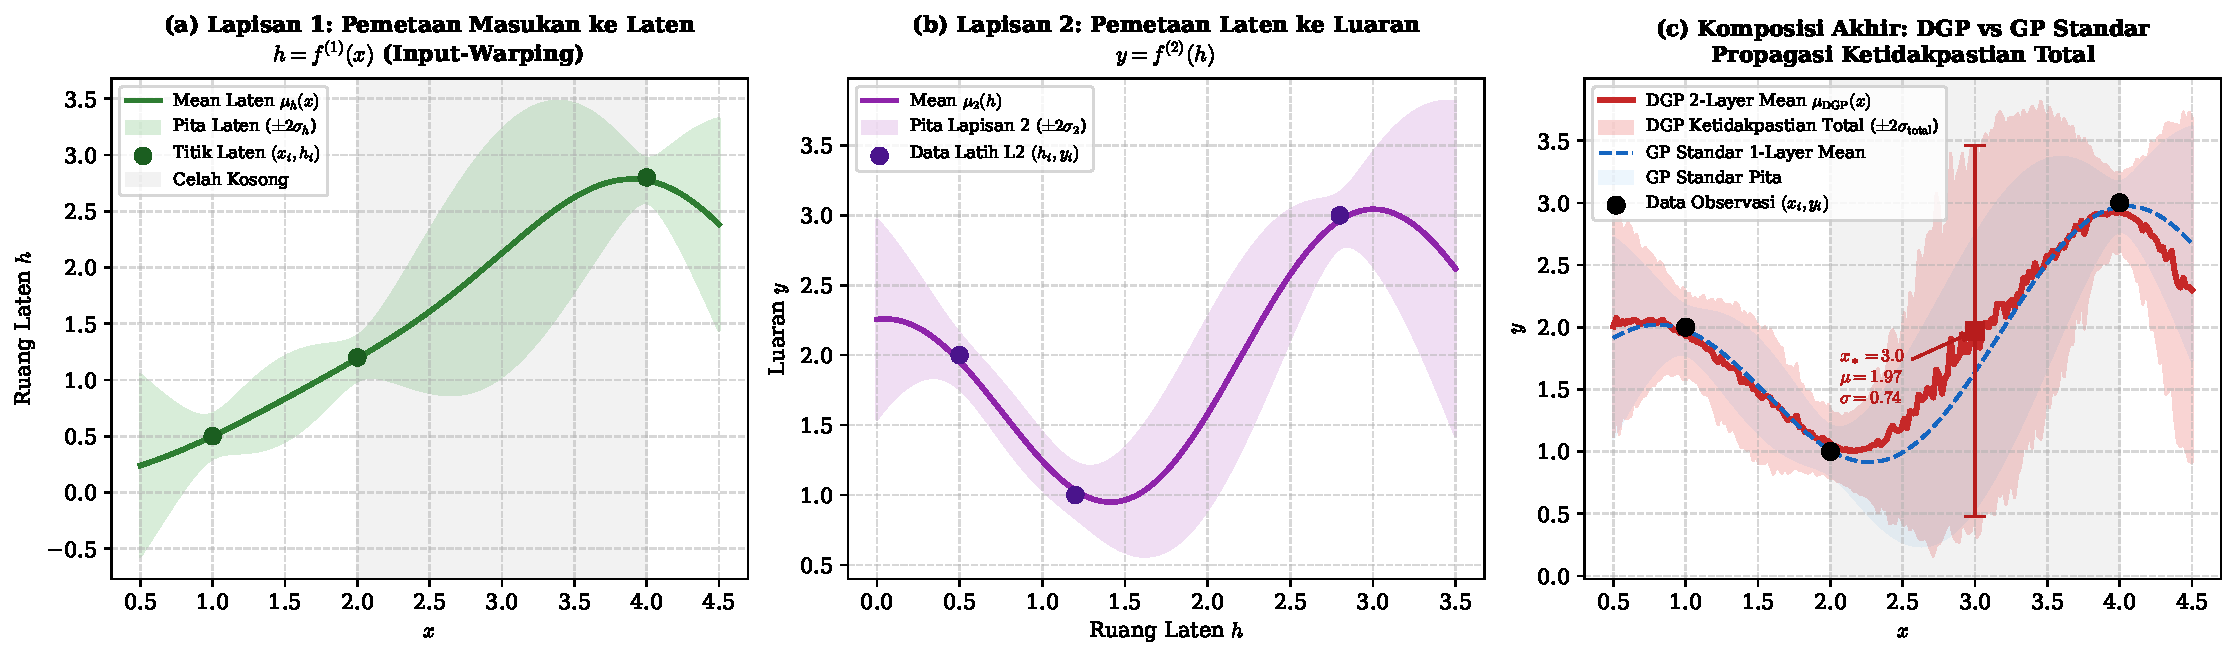
\includegraphics[width=0.70\textwidth]{dgp_toy_calculation.pdf}
\vspace{-0.3cm}
\caption{Visualisasi numerik DGP 2-Lapisan: (a) Pemetaan $x \to h$ (*input-warping*), (b) Pemetaan laten ke luaran $h \to y$, dan (c) Kurva akhir DGP dengan penggelembungan pita variansi di wilayah celah data kosong ($x_* = 3.0$).}
\label{fig:plot_dgp}
\end{figure}

\vspace{-0.3cm}
% =========================================================================
% SEKSI 4: PERBANDINGAN DAN RELEVANSI RISET
% =========================================================================
\section{Perbandingan dengan GP Standar dan Relevansi Tugas Akhir}
\label{sec:perbandingan}

\begin{table}[H]
\centering
\small
\renewcommand{\arraystretch}{0.95}
\caption{Perbandingan Metrik Prediksi pada Titik Interpolasi Celah ($x_* = 3.0$).}
\label{tab:komparasi}
\begin{tabularx}{\textwidth}{l>{\centering\arraybackslash}X>{\centering\arraybackslash}X>{\raggedright\arraybackslash}X}
\toprule
\textbf{Parameter Evaluasi} & \textbf{GP Standar (1-Lapis)} & \textbf{DGP (2-Lapis)} & \textbf{Makna Fisis \& Teoretis} \\
\midrule
Prediksi Mean ($\mu_*$) & $1.6388$ & $\mathbf{1.8931}$ & Mengakomodasi distorsi spasial non-stasioner \\
Variansi Lokal Luaran & $0.3002$ & $0.0616$ & Ketidakpastian kondisional Lapisan 2 \\
Variansi Merambat ($L_1$) & $0$ & $\mathbf{0.5636}$ & Fluktuasi fitur laten merambat ke luaran \\
Variansi Total ($\sigma_*^2$) & $0.3002$ & $\mathbf{0.6252}$ & Menggelembung 2x lipat (lebih realistis) \\
Standar Deviasi ($\sigma_*$) & $0.5479$ & $\mathbf{0.7907}$ & Estimasi ketidakpastian berjenjang yang jujur \\
\bottomrule
\end{tabularx}
\end{table}

\subsection{Analisis Komparatif: Mengapa Variansi DGP Membengkak?}
Dari perbandingan numerik pada Tabel~\ref{tab:komparasi}, terlihat perbedaan fundamental antara GP standar dan DGP:
\begin{enumerate}
    \item \textbf{Efek Distorsi Spasial (\textit{Input Warping})}: Prediksi mean DGP bergeser dari $1.6388$ ke $\mathbf{1.8931}$. Hal ini terjadi karena Lapisan 1 memetakan masukan $x_* = 3.0$ ke ruang laten dengan mean $\mu_{h*} = 2.1284$, yang secara relatif lebih condong mendekati titik latih $h_3 = 2.8$ dibandingkan posisi $x_*$ terhadap $x_3$ pada ruang masukan asli.
    \item \textbf{Penjumlahan Variansi Berjenjang}: Variansi total DGP menggelembung menjadi $\mathbf{0.6252}$ (dua kali lipat GP standar $0.3002$). Pada GP standar, ketidakpastian diasumsikan stasioner dan hanya fungsi dari jarak Euclidean masukan. Pada DGP, ketidakpastian dipecah menjadi dua: ketidakpastian kondisional Lapisan 2 ($0.0616$) dan ketidakpastian merambat dari fluktuasi representasi laten Lapisan 1 ($\mathbf{0.5636}$). Komponen kedua inilah yang mendominasi dan mencegah model menderita *overconfidence*.
    \item \textbf{Sifat Non-Gaussian Luaran}: Secara teoretis, distribusi marginal luaran DGP adalah campuran tak hingga (*infinite mixture*):
    \begin{equation}
        p(y_* \mid x_*, \mathcal{D}) = \int p\left(y_* \mid h_*, \mathcal{D}^{(2)}\right) p\left(h_* \mid x_*, \mathcal{D}^{(1)}\right) dh_*
    \end{equation}
    Integral ini menghasilkan distribusi posterior non-Gaussian yang mampu menangkap asimetri dan multimodalitas pada data kompleks.
\end{enumerate}

\subsection{Implikasi Metodologis untuk Tugas Akhir: \textit{Image Segmentation with DGP}}
Pada tugas akhir segmentasi citra, arsitektur DGP memberikan keunggulan metodologis yang signifikan:
\begin{itemize}
    \item \textbf{Ekstraksi Fitur Probabilistik}: \textit{Hidden layer} DGP bertindak sebagai ruang representasi fitur laten spasial. Jika GP standar terikat pada kernel stasioner kaku, DGP mampu meregangkan ruang laten di area transisi tajam dan merapatkannya di wilayah homogen.
    \item \textbf{Estimasi Batas Segmen Terkalibrasi}: Wilayah paling rawan galat pada segmentasi citra adalah piksel perbatasan antar-objek (\textit{boundary edges}). Di zona ambigu ini, komponen variansi laten merambat $\mathrm{Var}_{h_*}(\mathbb{E}[y_* \mid h_*])$ otomatis melonjak tinggi. Hal ini menghasilkan pita keyakinan yang lebar pada batas kontur objek, memberikan informasi ketidakpastian yang jujur bagi praktisi tanpa menderita prediksi yang keliru namun berkeyakinan tinggi (*overconfident misclassification*).
\end{itemize}

\end{document}
